\documentclass[letter, 10pt]{article}
\usepackage{fullpage}
\usepackage[margin=0.2in]{geometry}
\usepackage{graphicx}
\usepackage{wrapfig}
\usepackage{caption}
\usepackage{subcaption}
\usepackage{listings}
\usepackage{hyperref}
\usepackage{amsmath}
\usepackage{float}

\pagenumbering{gobble}

\begin{document}
\noindent
\large \textbf{Rahul Ghosh} \hfill \textbf{Assignment\#5}\\
\normalsize Student ID: 5476965 \hfill CSci 5561\\

\section*{\centering STEREO RECONSTRUCTION}

\subsection*{METHOD}
\subsubsection*{SIFT FEATURE MATCHING}
For the left and right image the sift features are extracted and matched using the ration test and bidirectional consistency, to get a set of corresponding points. The matched points are shown in Figure 1.

\subsubsection*{COMPUTING F}
Using the set of correspondences the F is computed by solving the following linear equation, where u and v are the features from the first and second image respectively. RANSAC is used to determine the F matrix, after which SVD cleanup is done to make it rank 2. 

\subsubsection*{RECTIFICATION HOMOGRAPHIES}
The rectification homographies for the left and right image are calculated such that the epipoles are at infinity. The warped left and right image are shown in Figure 2.

\subsubsection*{DISPARITY CALCULATION}
Using the warped left and right image the disparity is calculated after resizing the images to 0.2$\times$size.

\subsection*{RESULTS}

\begin{figure}[H]
    \minipage{0.48\textwidth}
        \centering
        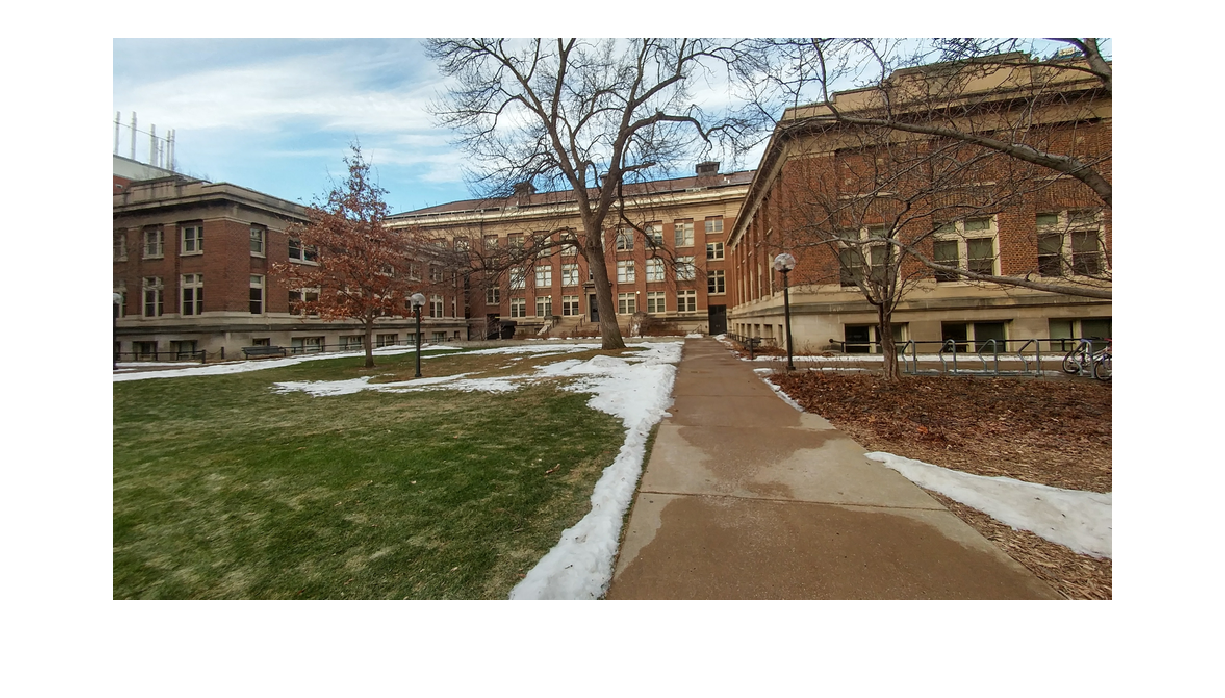
\includegraphics[width=\textwidth]{HW5/RESULT/im1.png}
        \subcaption{Left Image}
    \endminipage\hfill
    \minipage{0.48\textwidth}
        \centering
        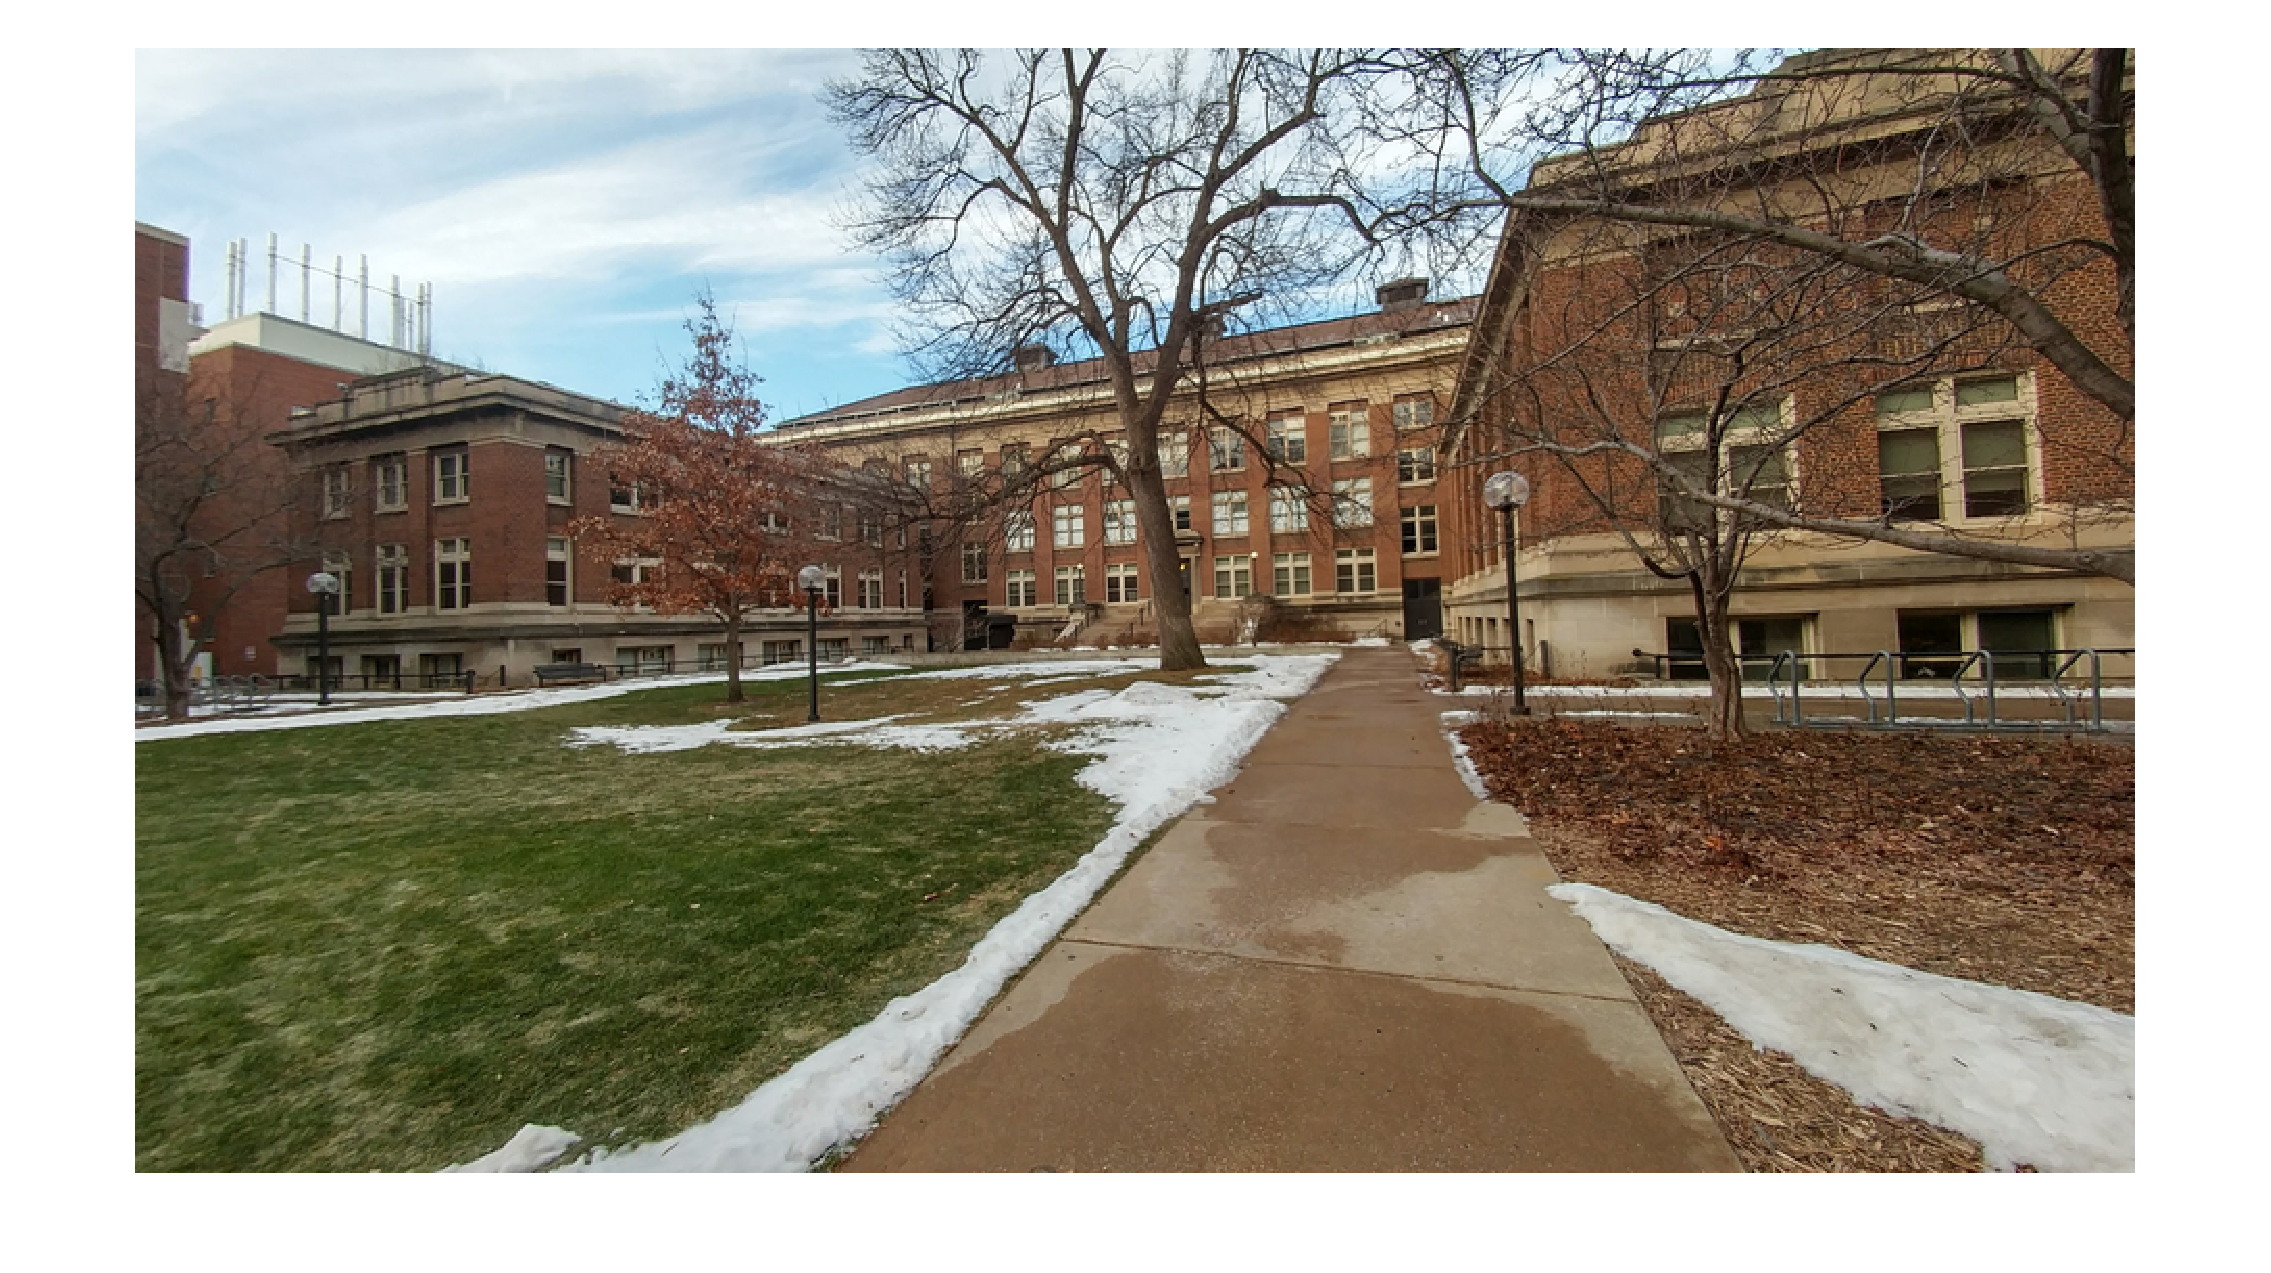
\includegraphics[width=1\textwidth]{HW5/RESULT/im2.png}
        \subcaption{Right Image}
    \endminipage\hfill
    \caption{Original Image}
\end{figure}

\begin{figure}[H]
    \centering
    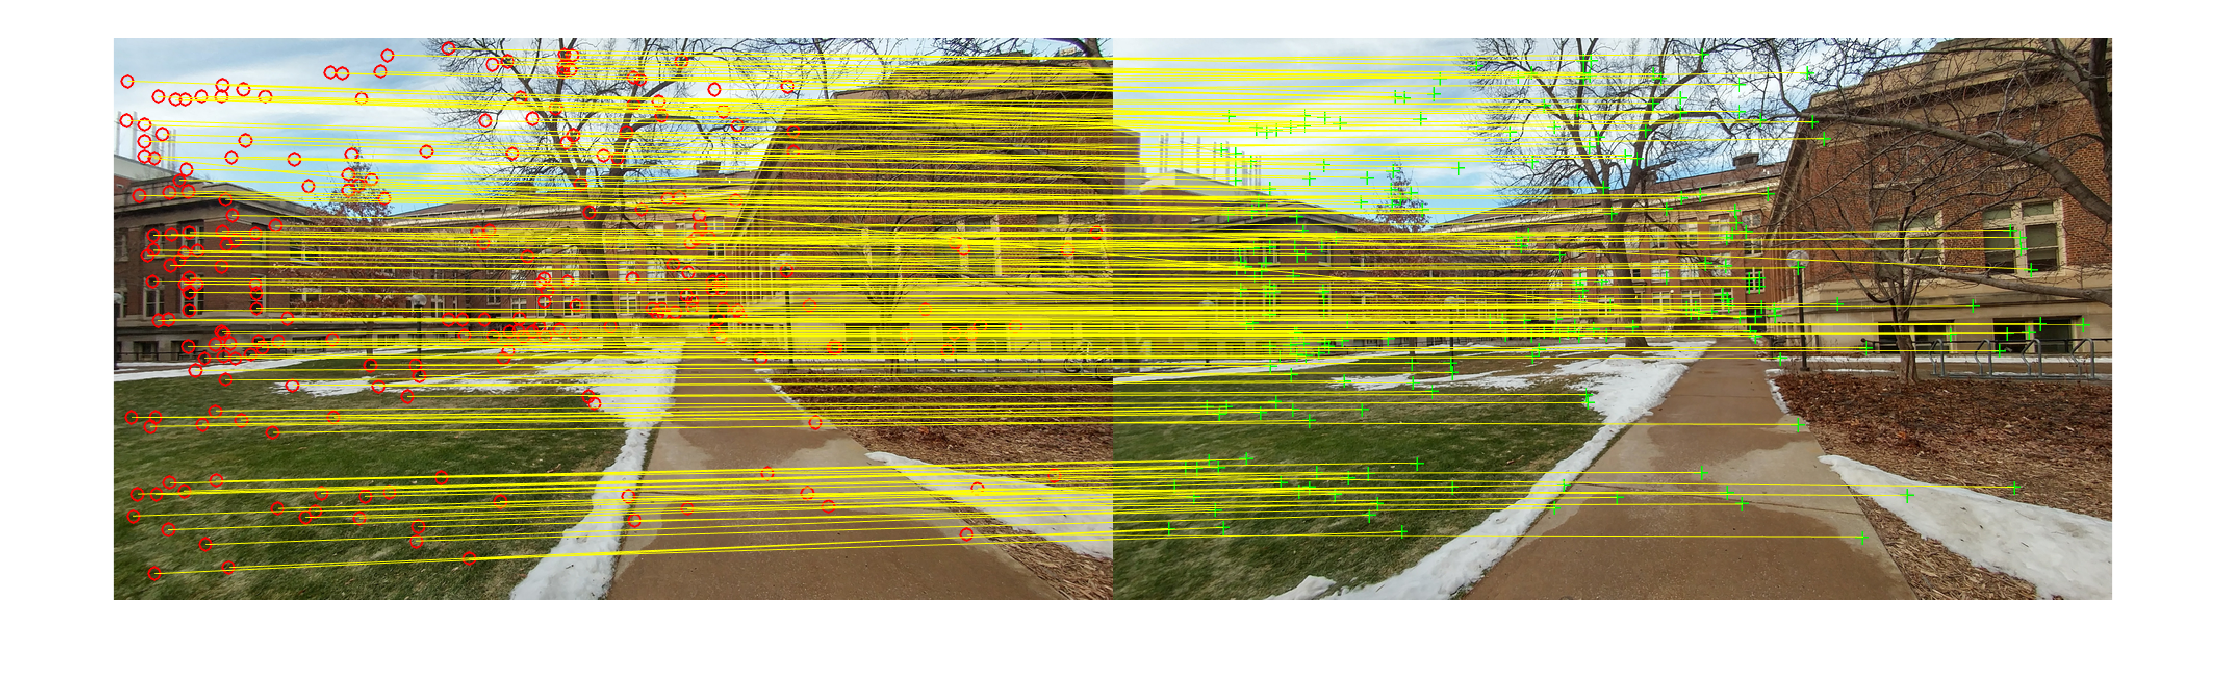
\includegraphics[width=\textwidth]{HW5/RESULT/matched_points.png}
    \caption{MATCHED POINTS}
    \label{fig:my_label}
\end{figure}

\begin{figure}[H]
    \minipage{0.48\textwidth}
        \centering
        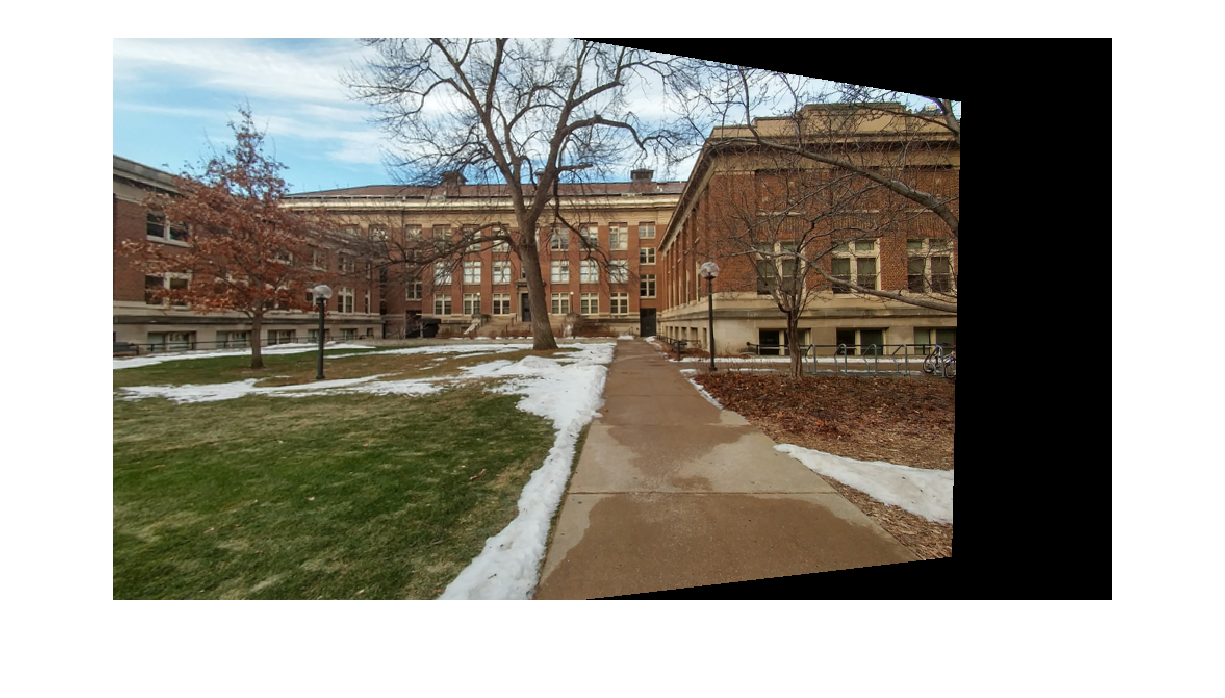
\includegraphics[width=\textwidth]{HW5/RESULT/im1_w.png}
        \subcaption{Left Rectified Image}
    \endminipage\hfill
    \minipage{0.48\textwidth}
        \centering
        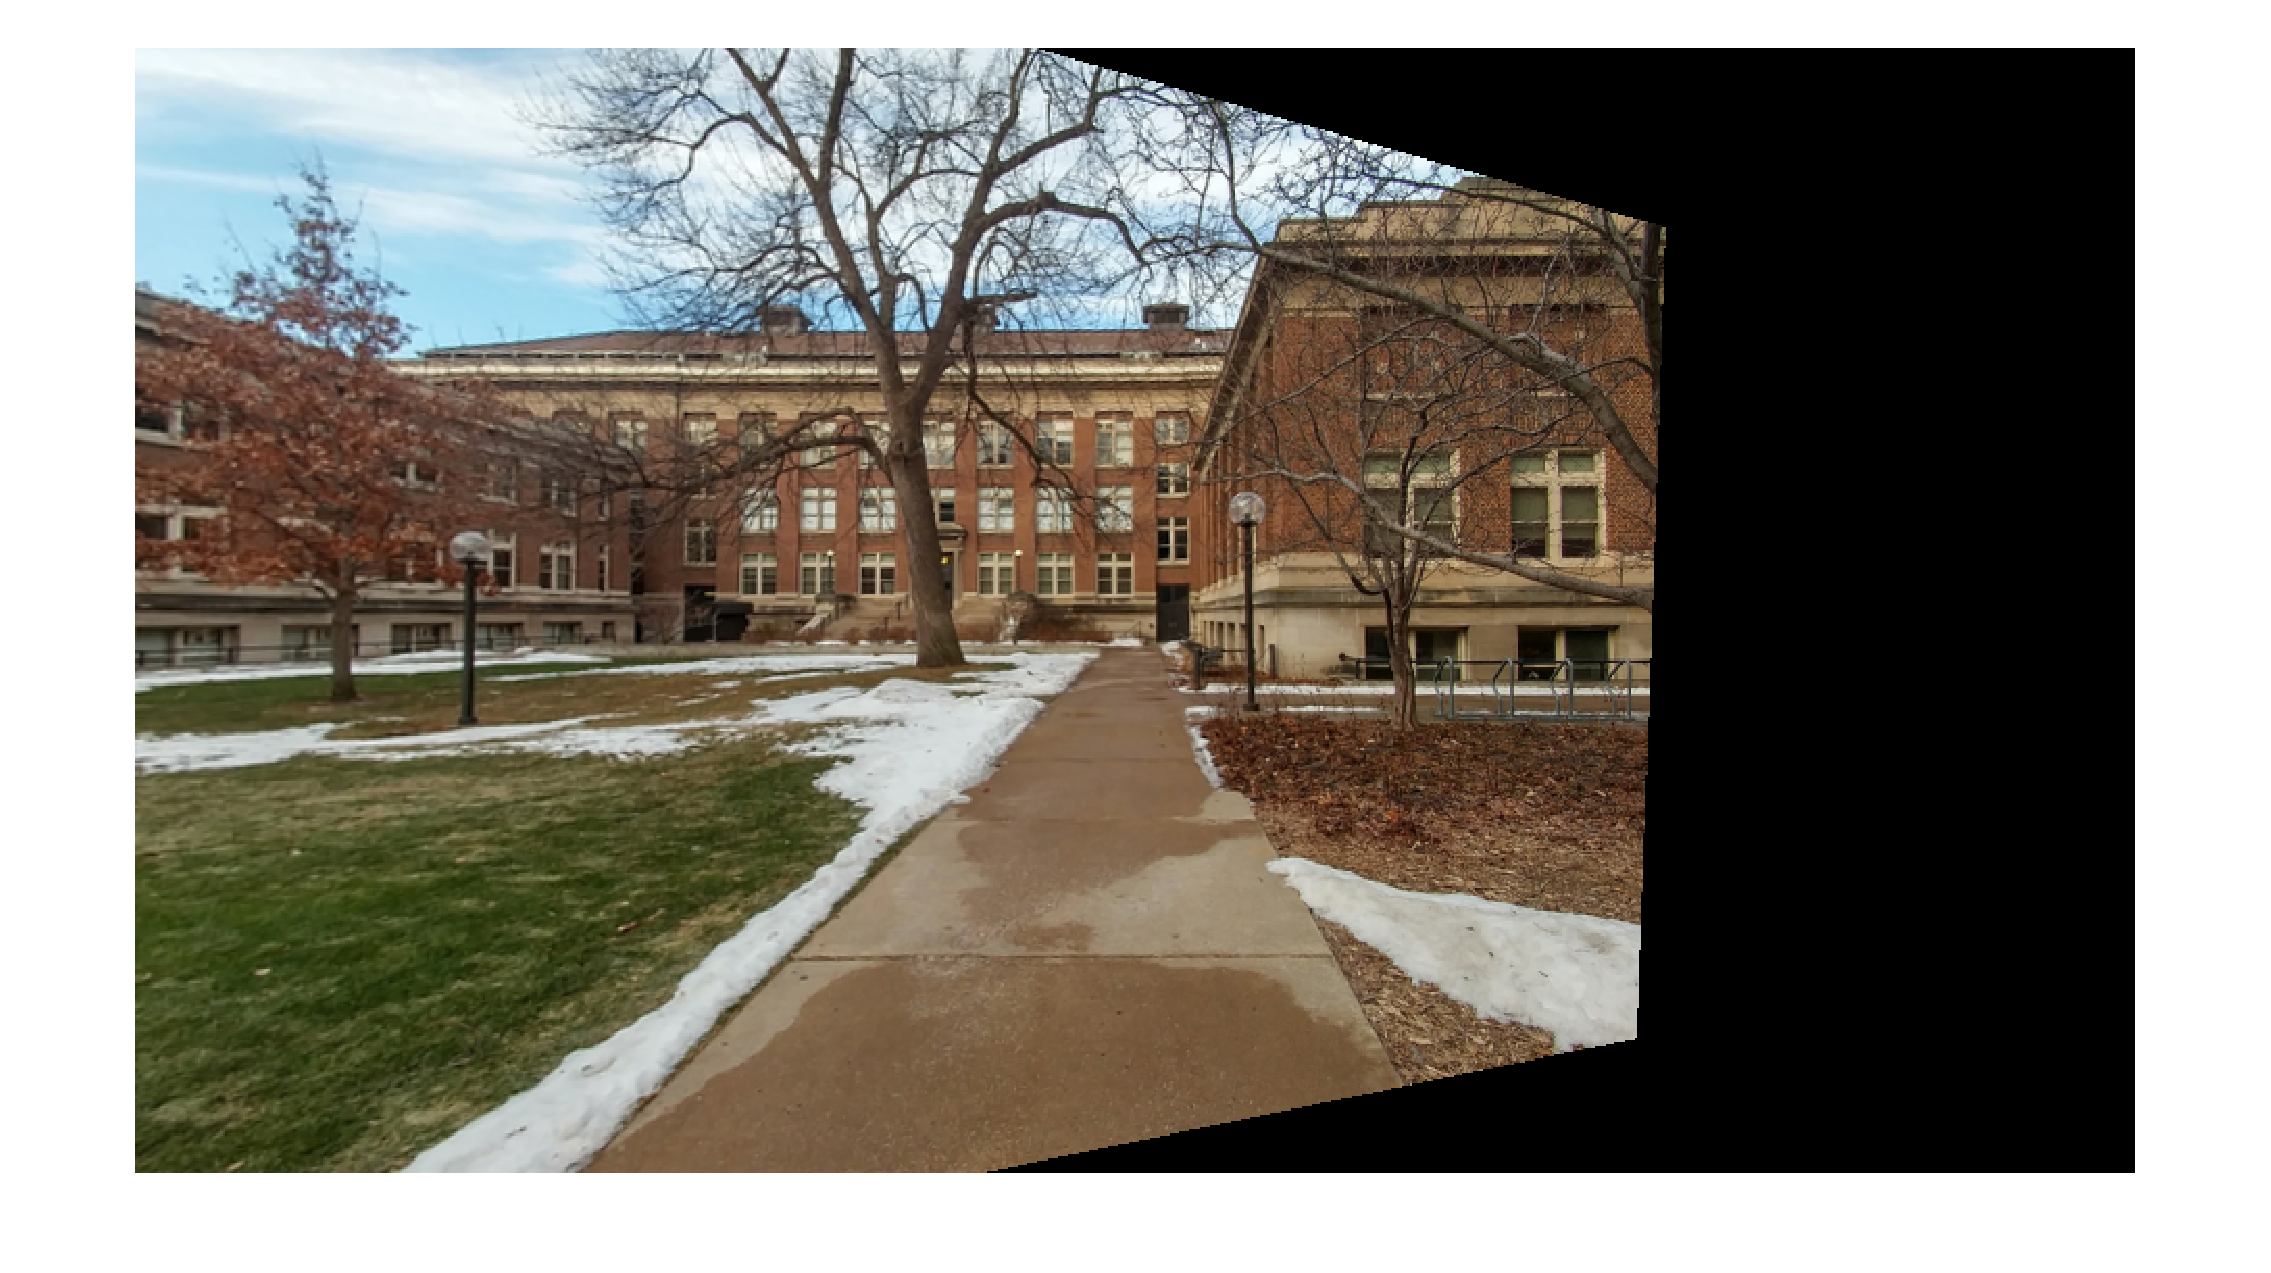
\includegraphics[width=\textwidth]{HW5/RESULT/im2_w.png}
        \subcaption{Right Rectified Image}
    \endminipage\hfill
    \caption{Rectified Image}
\end{figure}

\begin{figure}[H]
    \centering
    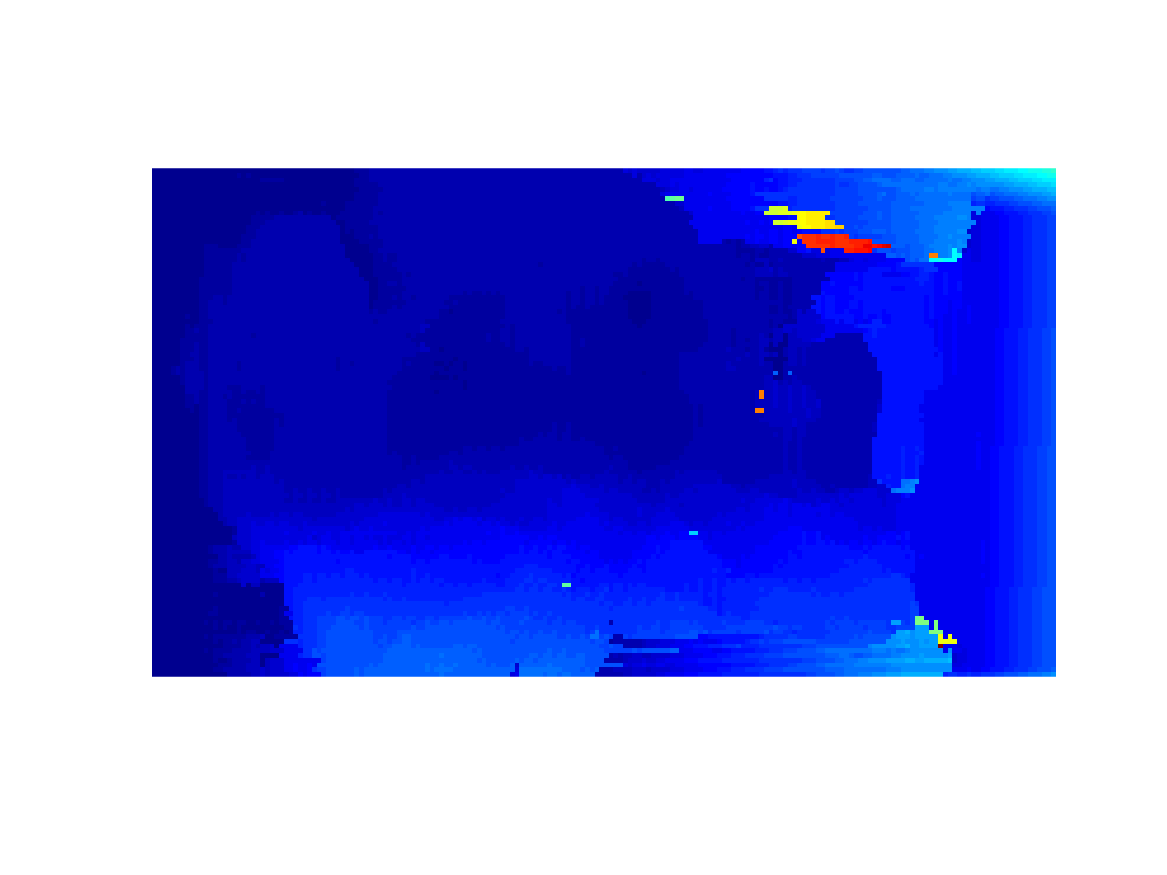
\includegraphics[width=\textwidth]{HW5/RESULT/disp.png}
    \caption{DISPARITY MAP}
    \label{fig:my_label}
\end{figure}

\end{document}